\begin{slide}
\heading{Concurrent datatypes}

A \emph{concurrent datatype} is a datatype (e.g.~a queue, stack, set or
mapping) that can be safely accessed concurrently by multiple threads.  

Threads that use the concurrent datatype can act much as they would with a
sequential datatype: the implementer of the threads does not need to think
much about concurrency.  

The implementer of the concurrent datatype \emph{does} have to think about
concurrency, and ensure different operation calls do not interfere with one
another.  But that concurrency is local, often inside a single object: local
reasoning is much easier than global reasoning.  And there's a lot of scope
for re-using concurrent datatypes.

Datatype-based concurrent programming encapsulates \emph{all} the concurrency
within a small number of concurrent datatypes.
\end{slide}

%%%%%

\begin{slide}
\heading{Example: a concurrent queue}

We will implement a concurrent queue.

What interface should a concurrent queue have?  A sequential queue would
typically have an interface like:

\begin{scala}
trait Queue[T]{
  /** Enqueue x. */
  def enqueue(x: T): Unit

  /** Dequeue a value.  
    * Pre: the queue is not empty. */
  def dequeue: T

  /** Is the queue empty? */
  def isEmpty: Boolean
}
\end{scala}
\end{slide}

%%%%% 

\begin{slide}
\heading{Example: a concurrent queue}

Client code is expected to check that the queue is non-empty before calling
|dequeue|:
\begin{scala}
  if(queue.isEmpty){ 
    ... // handle the empty queue
  } 
  else{ 
    val x = queue.dequeue; ... // do something with x
  }
\end{scala}

What happens if we use this approach  with a concurrent queue?
\end{slide} 

%%%%%


%% \begin{slide}
%% \heading{Example: a concurrent queue}

%% With the code on the previous slide, a thread~$A$ could call |queue.isEmpty|
%% and find that the queue is non-empty.  But before it performs the |dequeue|,
%% another thread could remove the last element from the queue.  Then when $A$
%% does perform the |dequeue|, the precondition is not satisfied.

%% This is sometimes called \emph{time-of-check to time-of-use} (TOCTTOU): there
%% is a gap between the check (that the queue is non-empty), and the operation
%% that depends upon that check (the dequeue), which means that the result of the
%% check may no longer be valid.
%% \end{slide}


%%%%%

\begin{slide}
\heading{Dealing with preconditions}

There are two main ways of dealing with operations that have a non-trivial
natural precondition.
%
\begin{itemize}
\item Return a special value to indicate that the natural precondition does
not hold.
\begin{itemize}
\item In Scala, it is natural to use an |Option| value, with |None| indicating
that the precondition does not hold.  
\item In some circumstances, it might be appropriate (and more efficient) to
use |null| for this, if |null| can never be returned when the precondition
does hold.
\item Throw an exception, and expect the thread to catch it.
\end{itemize}
%
Such operations are called \emph{total}. 

\item
If the precondition does not hold, block the thread until the precondition
becomes true.  Such operations are called \emph{partial}.
\end{itemize}
\end{slide}

%%%%% 


\begin{slide}
\heading{A total queue}

We will implement a total concurrent queue, with the following interface.
%
\begin{scala}
/** A total queue. */
trait TotalQueue[T]{
  /** Enqueue x. */
  def enqueue(x: T): Unit

  /** Dequeue a value.  Returns None if the queue is empty. */
  def dequeue: Option[T]

  /** Shut down the queue. */
  def shutdown: Unit
}
\end{scala}
\end{slide}

%%%%%

\begin{slide}
\heading{Dealing with preconditions}

Threads performing a |dequeue| should do something like
\begin{scala}
  queue.dequeue match{
    case Some(x) => ... // do something with x
    case None => ... // handle the empty queue
  }
\end{scala}
\end{slide}

%%%%%

\begin{slide}
\heading{Encapsulating a server}

We will implement the concurrent queue by encapsulating a server process.
But we could also implement the queue using one of the techniques we'll see
later in the course.

The server will store the queue itself (using a |Queue| from the Scala API).
Clients will use channels to cause the server to enqueue and dequeue values.

\begin{scala}
class ServerTotalQueue[T] extends TotalQueue[T]{
  // Channels used for enqueueing and dequeueing.
  private val enqueueChan = new SyncChan[T]
  private val dequeueChan = new SyncChan[Option[T]]

  def enqueue(x: T) = enqueueChan!x

  def dequeue: Option[T] = dequeueChan?()
  ...
}
\end{scala}
\end{slide}

%%%%%

\begin{slide}
\heading{Encapsulating a server}

\begin{scala}
  private def server = thread{
    val queue = new scala.collection.mutable.Queue[T]
    serve(
      enqueueChan =?=> { x => queue.enqueue(x) }
      | dequeueChan =!=> { if(queue.nonEmpty) Some(queue.dequeue) else None }
    )
  }

  server.fork

  def shutdown = { enqueueChan.close; dequeueChan.close }
\end{scala}

Note that the server handles operations in a one-at-a-time way, preventing
operations from interfering with one another.

Note also that calling |shutdown| is necessary to ensure the server thread
terminates; this will also allow garbage collection. 
\end{slide}


%% %%%%%

\begin{slide}
\heading{Exercise}

Implement a total concurrent stack using a similar technique.
\end{slide}

%%%%%

\begin{slide}
\heading{Correctness}

What does correctness mean for a concurrent queue?
%% How can we test concurrent queue implementations?
%% We need first to be clear about what correctness means. 
\begin{itemize}
\item Each operation should take place (apparently) in a one-at-a-time way,
without interference between operations.  

\item The point at which each operation takes effect is between the time the
operation was invoked and when it returns.  

\item The values returned by operations should be the same as for a sequential
queue (when the operations are performed in the same order). 
\end{itemize}

This property is called \emph{linearization}.  The points at which operations
appear to take effect are called \emph{linearization points}.  (See the
Concurrent Algorithms and Data Structures course for a formal definition.)
\end{slide}

%%%%%%

%% \begin{slide}
%% \heading{Correctness}

%% With the server-based queue, each operation appears to take place at the point
%% of the corresponding channel communication.  This communication is between the
%% call and return of the operation.  The server ensures the values are
%% compatible with this order of the operations.
%% \end{slide}

%% %%%%%

\begin{slide}
\heading{Linearization examples}

In the timeline below, the dequeue of 4 can be explained by the operations
being linearized at the points marked ``X''.
%
\unScalaMid
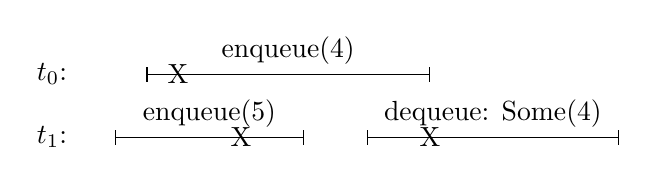
\begin{tikzpicture}[scale=0.8]
\draw (0,0) node {$t_0$:}; 
\draw[|-|] (1.5,0) -- node[above] {\scalashape enqueue(4)} (6,0);
\draw(2,0) node{X};
\draw (0,-1) node {$t_1$:}; 
\draw[|-|] (1,-1) -- node[above] {\scalashape enqueue(5)} (4,-1);
\draw(3,-1) node{X};
\draw[|-|] (5,-1) -- node[above] {\scalashape dequeue: Some(4)} (9,-1);
\draw(6,-1) node{X};
\end{tikzpicture}


Note that the history
\begin{scala}
  enqueue(4), enqueue(5), dequeue: Some(4)
\end{scala}
would be valid on a corresponding sequential queue. 
\end{slide}

%%%%%

\begin{slide}
\heading{Linearization examples}

But with different linearization points, a dequeue of 5 might have happened.

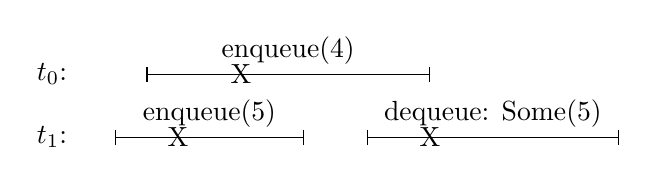
\begin{tikzpicture}[scale=0.8]
\draw (0,0) node {$t_0$:}; 
\draw[|-|] (1.5,0) -- node[above] {\scalashape enqueue(4)} (6,0);
\draw(3,0) node{X};
\draw (0,-1) node {$t_1$:}; 
\draw[|-|] (1,-1) -- node[above] {\scalashape enqueue(5)} (4,-1);
\draw(2,-1) node{X};
\draw[|-|] (5,-1) -- node[above] {\scalashape dequeue: Some(5)} (9,-1);
\draw(6,-1) node{X};
\end{tikzpicture}

Again note that the history
\begin{scala}
  enqueue(5), enqueue(4), dequeue: Some(5)
\end{scala}
would be valid on a corresponding sequential queue. 
\end{slide}

%%%%%

\begin{slide}
\heading{Linearization examples}

With the following timeline, the dequeue must return 5: any other return would
not be linearizable.
%
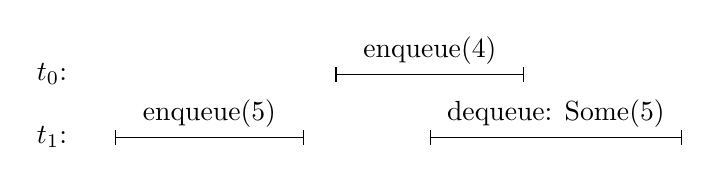
\begin{tikzpicture}[scale=0.8]
\draw (0,0) node {$t_0$:}; 
\draw[|-|] (4.5,0) -- node[above] {\scalashape enqueue(4)} (7.5,0);
%\draw(3,0) node{X};
\draw (0,-1) node {$t_1$:}; 
\draw[|-|] (1,-1) -- node[above] {\scalashape enqueue(5)} (4,-1);
%\draw(2,-1) node{X};
\draw[|-|] (6,-1) -- node[above] {\scalashape dequeue: Some(5)} (10,-1);
%\draw(6,-1) node{X};
\end{tikzpicture}

And the following history is not linearizable, because the queue is non-empty
throughout $t_2$'s operation.
%
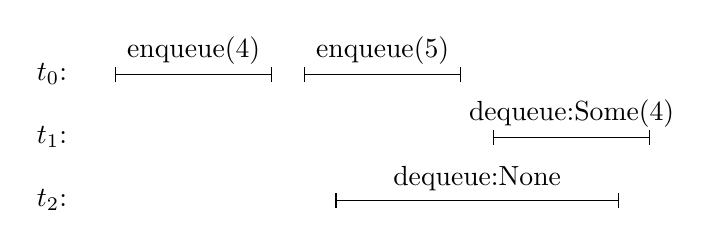
\begin{tikzpicture}[scale=0.8]
\draw (0,0) node {$t_0$:}; 
\draw[|-|] (1,0) -- node[above] {\scalashape enqueue(4)} (3.5,0);
\draw[|-|] (4,0) -- node[above] {\scalashape enqueue(5)} (6.5,0);
\draw (0,-1) node{$t_1$:};
\draw[|-|] (7,-1) -- node[above] {\scalashape dequeue:Some(4)} (9.5,-1);
\draw (0,-2) node{$t_2$:};
\draw[|-|] (4.5,-2) -- node[above] {\scalashape dequeue:None} (9,-2);
\end{tikzpicture}
\scalaMid
\end{slide}

%%%%%


%%%%%

\begin{slide}
\heading{Synchronous channels}

It is important that we use \emph{synchronous channels} in the server-based
queue.  Suppose we used buffered channels.  Then the following behaviour is
possible.
%
\begin{enumerate}
\item Thread $t_1$ calls |enqueue(5)|, but the value~|5| stays in the
  |enqueueChan|, even after $t_1$ returns;

\item Thread $t_2$ calls |dequeue|, and the server sends it |None|.
\end{enumerate}

Alternatively
%
\begin{enumerate}
\item The server sends |None| on |dequeueChan|, and that value stays in the
  channel; 

\item Thread $t_1$ calls |enqueue(5)|, and this value is received and stored
  by the server; 

\item Thread $t_2$ calls |dequeue|, and receives the |None| sent earlier.
\end{enumerate}
\end{slide}

%%%%%

\begin{slide}
\heading{Synchronous channels}

Using synchronous channels, the operations have an effect in the order of the
channel communications.  This order is compatible with the order of the
operation calls and returns.

We will always use synchronous channels when implementing a concurrent
datatype using a server process.   
\end{slide}


%%%%%

\begin{slide}
\heading{Testing for linearizability}

How can we test for linearizability?

Basic idea: 
%
\begin{itemize}
\item Run some threads on the concurrent queue, performing random |enqueue|
and |dequeue| operations, and record the history of operation calls and
returns;

\item Search for a corresponding sequential history that explains
linearizability, and that is a valid history for the corresponding sequential
datatype.  If none is found, signal an error.
\end{itemize}
%
Repeat many times.
\end{slide}

%%%%%

\begin{slide}
\heading{Testing for linearizability}

I've developed a framework to support such testing\footnote{{Testing
    for Linearizability}, Gavin Lowe, \textit{Concurrency and Computation},
    Practice and Experience, 29 (4), 2017,
  \url{http://www.cs.ox.ac.uk/people/gavin.lowe/LinearizabiltyTesting/}.},
and, in particular, investigated algorithms for testing whether a concurrent
history is linearizable.

In the next slides, we'll see a stripped-down testing script that uses this
(the full version can be used with multiple concurrent queue implementations,
and replaces the numerical constants by variables, specifiable via the command
line).

\vfill
\end{slide}

%%%%%

\begin{slide}
\heading{A small testing script}

The test program works on a concurrent datatype of some type~|C|; here we use
a |TotalQueue| containing |Int|s.  The test program
also requires a corresponding, \emph{immutable, deterministic}
sequential specification datatype~|S|, here an immutable queue from the Scala
API.
%
\begin{scala}
object QueueTest{
  type C = TotalQueue[Int]
  type S = scala.collection.immutable.Queue[Int]
  ...
}
\end{scala}
\end{slide}

%%%%%

\begin{slide}
\heading{A small testing script}

For each operation |op : A| on the concurrent datatype, we need a
corresponding function |seqOp : S => (A, S)| on the sequential datatype, which
returns the same value as the concurrent operation\footnote{More precisely,
  the two values should be equal, as tested using the ``{\scalashape ==}''
  method.}, paired with the new value of the sequential datatype.  These are
normally simple wrappers around API code.
%
\begin{scala}
  def seqEnqueue(x: Int)(q: S) : (Unit, S) = ((), q.enqueue(x))
  def seqDequeue(q: S) : (Option[Int], S) =   
    if(q.isEmpty) (None, q) 
    else{ val (r,q1) = q.dequeue; (Some(r), q1) }
\end{scala}
\vfill
\end{slide}

%%%%%

\begin{slide}
\heading{A small testing script}

The main part of the test program is the definition of a |worker| function
that performs and logs operations on the concurrent datatype, associating each
concurrent operation with a corresponding operation on the sequential
datatype.  Here, the worker performs 200 operations; each is (with probability
0.3) an enqueue of a random value, or (with probability~0.7) a dequeue.
\begin{scala}
  def worker(me: Int, log: LinearizabilityLog[S, C]) = {
    val random = new scala.util.Random
    for(i <- 0 until 200)
      if(random.nextFloat <= 0.3){
        val x = random.nextInt(20)
        log(_.enqueue(x), s"enqueue($x)", seqEnqueue(x))
      }
      else log(_.dequeue, "dequeue", seqDequeue)
  }
\end{scala}
\end{slide}

%%%%%

\begin{slide}
\heading{A small testing script}

The worker takes a log object |log| as a parameter; each operation is
performed and logged via a call to |log|, taking three parameters:
%
\begin{itemize}
% \item
% The identity of the thread doing the operation;

\item
The operation to be performed on the concurrent datatype;

\item A string describing the operation (this is used in debugging output in
the case that a non-linearizable history is found, and is also used internally
for optimisations; semantically different operations should have different
strings);

\item
The corresponding operation on the sequential datatype.
\end{itemize}

The call to |log| logs the invocation of the concurrent operation,
performs the concurrent operation, and logs the result returned.
\end{slide}
\begin{slide}
\heading{A small testing script}

The main test for linearizability is performed at line~\ref{line:maintest},
below, repeated so as to consider 1000 histories.  The  tester
takes as arguments: the sequential datatype; the concurrent datatype; the
number |p| of worker threads to run; and the definition of a worker thread.
%
\begin{scala}[numbers=left,numberstyle=\scriptsize]
  def main(args: Array[String]) = for(i <- 0 until 1000){
    val concQueue = new ServerTotalQueue[Int] // The concurrent queue
    val seqQueue = Queue[Int]() // The sequential specification queue
    val tester = LinearizabilityTester[S, C](seqQueue, concQueue, 4, worker _)
    assert(tester() > 0)£\label{line:maintest}£
  }
\end{scala}
%
The linearizability tester runs |p| workers concurrently, logging the
operation calls on the concurrent datatype.  It then tests whether the
resulting history is linearizable, returning a positive result if so.
\end{slide}

%%%%%

\begin{slide}
\heading{Controlling the search space}

The algorithm for testing linearizabilty, in effect, considers all possible
linearizations of the history, i.e.~all ways of ordering the operations
consistent with the history.  It then tests whether that ordering is
compatible with the sequential datatype, i.e.~whether performing the
corresponding sequential operations in the same order would give the same
results. 

Thus the algorithm considers all  states that the sequential
specification object could get into after a prefix of such linearizations.
%
If there are too many such states, this will take a long time.  It's therefore
a good idea to design the test so that such bad cases are very unlikely.
\end{slide}

%%%%%

\begin{slide}
\heading{Controlling the search space}

With a queue, the linearizability tester considers all possible states of the
sequential queue formed by permuting concurrent enqueue operations.  This
number grows exponentially with the length of the queue.  We therefore try to
avoid the length of the queue growing too much.  We did this in the earlier
testing harness by making dequeues more frequent than enqueues.
\end{slide}

%%%%%

\begin{slide}
\heading{Logging}

By default, the linearizability tester logs operation calls using thread-local
logs, pairing each event with a timestamp.  We saw a similar technique in an
earlier chapter.  If you're using an operating system that doesn't support
timestamps property, setting the optional parameter |tsLog| to |false| will
use a different type of log. 
%
\begin{scala}
  val tester = LinearizabilityTester[S, C](
    seqQueue, concQueue, 4, worker _, £\scalastyle\color{red} tsLog = false£)
\end{scala}
\end{slide}

%%%%%

%% \begin{slide}
%% \heading{Exercise}

%% Implement and test a total concurrent stack using similar techniques.
%% \end{slide}
